\section{General Information}

This document is intended as a template and guideline and should support the author in the course of doing the master's thesis.
Assessment criteria comprise the quality of the theoretical and/or practical work as well as structure, content and wording of the written master's thesis. Careful attention should be given to the basics of scientific work (e.g., correct citation).

\section{Introduction}
Navigation and planning are essential for mobile robots to act in out- and indoor environments. 
Uncountable articles are describing approaches and applied solutions of autonomous system driving safely in different domains, e.g. Stanley \cite{stanley} a self driving car that won the DARPA Grand Challenge by driving 132~miles through the Mojave desert, or the mobile robots of Kiva Systems \cite{kiva} handling goods in distribution centers and warehouses like Amazon. 
Articles like \cite{stanley} and \cite{kiva} present the relationship between the environmental complexity and the computational on-board power needed to deal with it.
Stanley has a six processor computing platform sponsored by Intel whilst Kiva robots are using low cost DSP's for navigation and vision processing\footnote{Kiva Systems Uses "Smart" Blackfin-powered Robots for Warehouse Navigation | Analog Devices: \url{http://www.analog.com/en/content/kiva_systems_bf548/fca.html}} to drive within a known environment. 
The robot shown in Figure~\ref{fig:fig_pioneer} is used on our institute. The robot is able to drive autonomous within our lab/office environment and is equipped with one Intel processor (i5@3,4GHz) running Robotic Operation System (ROS)\footnote{Robot Operating System (ROS): \url{http://ww.ros.org/}}.  
While the application domain and computational power varies strongly between the robotic systems, all of them have to move safely and efficient from one location to another. 

   \begin{figure}[thpb]
      \centering
      \def\svgwidth{0.7\textwidth}
      \includesvg{figures/pioneer_costmap}
      \caption{This figure shows a Pionner3DX and its view of the office environment while passing through a door. The blue line shows the global path and the green line the selected trajectory of the local planner.}
      \label{fig:fig_pioneer}
   \end{figure}

A common strategy to deal with the complex planning problem is the division into a global and a local planning problem \cite{LaValle2006}.
Global path-planning requires a simplified representation, e.g. static map, of the search problem to efficiently compute an optimal shortest path using variants of Dijkstra's \cite{dijkstra1959note} or $A^*$ \cite{DBLP:journals/tssc/HartNR68/Astar} algorithm, ignoring kinematic and acceleration constraints of the robot.
In succession the retrieved global path is used by a local planner for guiding the robot through the environment.
%(REMARK: global path planning in la valle, D*, FD* usw. eventuel)%
The local planner takes sensor readings of the robot into account and is reactive to changes within the sensor range. 
It chooses the best values of available motor controls in respect to the kinematic and dynamic constraints of the robot. 
The main task is to avoid collision with obstacles, by generating feasible velocity commands to produce a trajectory for the robot near the global path.
The heuristic strategy presented optimizes the local planner.   

One of the most popular local planer and reactive collision avoidance method is the Dynamic Window Approach (DWA)\cite{DWA1997}. Its based on evaluating a fixed number of trajectory samples in a reduced velocity space. 
A dynamic window around the current robot fused with the current sensor readings of the robot represents a so called costmap.
Trajectories are sampled into that costmap and weighted by a cost function.
Recent adoptions of this method can be found in \cite{conf/icra/SederP07}\cite{DBLP:conf/icra/Marder-EppsteinBFGK10}
%(REMARK: Other methods with fixed sized samples: Curvatur Velocity Method. Lane curvature method, lookup sources, cite resent papers which use this apporaches)

In this paper we propose a method which finds the best velocity commands by using search strategies based on Meta-Heuristics instead of evaluating a fixed number of trajectories in a brute force manner.
A combination of Iterated Local Search (ILS) with different neighborhood structures, Variable Neighborhood Search (VNS), and a Tabu list provides a significant documented performance boost. 

This enables the local planer to:
\begin{itemize}
\item run at a higher frequency
\item simulate trajectories for a longer time interval
\item moving the robot at higher speed
\item investigate a larger amount of trajectories
\item use a higher costmap resolution
\end{itemize}

The next section presents related work, followed by a detailed description of the approach in Section~\ref{sec:Approach}, and results of the experiments are given in Section~\ref{sec:testresults}. 
\section{Related Work} \label{sec:RelatedWork}
Of particular interest are local planning methods which apply sampling and simulation of trajectories. 
Here the maximization step can easily be substituted by the proposed method. The next two section describe the recent developments of this family of planners and gives an introduction to the used Meta-Heuristic algorithm.

\subsection{Local Planning and Obstacle Avoidance}
A well known method for local planning is the Dynamic Window Approach proposed in \cite{DWA1997}. 
The method discretely samples the velocity space $(v,w)$ of the robot, where $v$ is the \emph{linear velocity} and $w$ the \emph{angular velocity} of the robot, to create a set of feasible trajectories.
The velocity space is reduced to the reachable minimal and maximal velocity in one control cycle, taken the acceleration limits of the robot into account.
For a fixed amount of velocity samples the corresponding trajectories are created using a predefined granularity by performing forward simulation for a short period of time, starting at the current position of the robot. Evaluating all trajectories with respect to a weighted cost function (cf. Equation~\ref{eq:costfunction}) identifies the best trajectory.

\begin{equation}
   f_c(v,w)=\alpha f_a(v,w)+\beta f_d(v,w)+\gamma f_v(v,w)
   \label{eq:costfunction}
\end{equation}

The function $f_a(v,w)$ judges the angle between the robots heading and a given goal position.
It is maximal if the heading is a straight line to the goal.
The distance to the closest obstacle is calculated in the function $f_d(v,w)$.
The function $f_v(v,w)$ takes the forward velocity into account and rewards faster movements of the robot.
This method does not use a global plan to guide the robot, so without further changes it is subject to get captured in local minima.

Other applications of this approach in recent planning systems, adapt the corresponding cost function. 
%give some recent papers about dwa in developments%
The excellent \texttt{move\_base}\footnote{move\_base planning framework: \url{http://wiki.ros.org/move_base}} motion-planning framework introduced in \cite{DBLP:conf/icra/Marder-EppsteinBFGK10} implements within the navigation stack of Robot Operating System (ROS) local planner which incorporate global plans.

One implementation is based on DWA.
There is also the option to use Trajectory rollout \cite{gerkey08planning} as a local planner which is very related to the DWA, but in contrast improves in simulating the robots trajectory by accurately applying acceleration limits over the whole simulation time.
The cost function maximizes characteristics like proximity to obstacles, proximity to the goal, proximity to the global path, and speed.
Furthermore a number of escaping strategies try to avoid the vulnerability to local minima. 

Collision detection and cost calculation is performed by using the footprint of the robot following the calculated trajectory.
Hence the discretized footprint, which is usually given as a simple polygon, is projected on the costmap. 
Bresenham's Line algorithm \cite{bresenham1965algorithm} is used for ray-tracing the contour of a robot in the discrete workspace. 
Figure~\ref{fig:fig_global} shows the global view of the planning task. 
In Figure~\ref{fig:fig_local} the corresponding local view is depicted, including all sampled trajectories which are evaluated using a local costmap.

\begin{figure}[thpb]
      \footnotesize
      \centering
    \begin{subfigure}[]{0.35\textwidth}
      \centering
      \def\svgwidth{0.8\textwidth}
      \includesvg{figures/fig_global}
      \caption{Path planning in global costmap.}
      \label{fig:fig_global}
    \end{subfigure}
   \begin{subfigure}[]{0.35\textwidth}
      \centering
      %\def\svgscale{0.33}
      \def\svgwidth{0.8\textwidth}
      \includesvg{figures/fig_local}
      \caption{Trajectory generation for linear, and angular velocities $(v,w)$ in local costmap guided by global path.}
      \label{fig:fig_local}
   \end{subfigure}
   \caption{}
   \label{fig:fig_overview}
\end{figure}

%    \begin{figure}[thpb]
%      \footnotesize
%      \centering
%      \def\svgscale{0.65}
%      \includesvg{figures/fig_global}
%      \caption{Path planning in global costmap.}
%      \label{fig:fig_global}
%   \end{figure}
%
%   \begin{figure}[thpb]
%      \footnotesize
%      \centering
%      \def\svgscale{0.33}
%      \includesvg{figures/fig_local}
%      \caption{Trajectory generation for linear, and angular velocities $(v,w)$ in local costmap guided by global path.}
%      \label{fig:fig_local}
%   \end{figure}

Concerning the optimization of the used cost functions the most common approach for DWA and related local planner is to evaluate all possible trajectories in a reduced discrete velocity space. 
Examples of this approach can be found in \cite{kiss2012advanced}\cite{DBLP:conf/icra/Marder-EppsteinBFGK10}\cite{conf/icra/SederP07}. 

The Curvature Velocity Method in \cite{simmons1996curvature} considers approximation techniques like simulated annealing to maximize the cost function using the whole velocity space, but abandoned the idea due to still high computational costs. 
Instead of using discrete samples of the velocity space, it divides the space in sets of curvature intervals. 
Evaluation is performed by evaluating over all curvature intervals.

The proposed method extends the DWA approach, by using approximation algorithm to maximize the cost function in a discrete representation of the velocity space.

\subsection{Meta-Heuristic Search}
The family of algorithm using Meta-Heuristics is extremely successful in solving combinatorial problems (e.g. Traveling Salesman problem, MAX-Sat problem, scheduling problems). 
These algorithm build on the idea of executing multiple searches to find local optimal solutions in different parts of the search space using randomization, which together yield a global approximate optimal solution.

The basic Local Search (LS) (cf. Algorithm~\ref{localsearchalgo}) finds a local optimum according to a cost function $cost(x)$ and a fixed sized region around an initial solution in the solution space. 
The set of solutions in this region is denoted as the neighborhood of $x$. The necessary steps to get from the initial solution to a solution in the neighborhood is called a move.
\begin{algorithm}
\caption{Local Search  (LS)}
\label{localsearchalgo}
\begin{algorithmic} 
\State $x\gets$ initial solution
\Repeat
\State select a $x^\prime \in$ \Call{Neighborhood}{$x$}
\If {\Call{$cost$}{$x^\prime$} $\leq$ \Call{$cost$}{$x$}}
    \State $x\gets x^\prime$
\EndIf
\Until{stopping criteria satisfied}
\end{algorithmic}
\end{algorithm}

A nice survey of Iterative Local Search including the basic algorithm (cf. Algorithm~\ref{ilsalgo}) can be found in \cite{lourencco2001iterated}. 
The main idea is to call a local search procedure iteratively, until a certain stopping criteria is satisfied. 
In each iteration the current solution might be perturbed by changing parts of the solution. 
The following local search takes this altered solution as a starting point and returns a new solution. 
If it satisfies an acceptance condition (e.g. the best solution so far), the process restarts with the new solution. 
In addition, a history of already found solutions may be used to steer perturbation and the acceptance test.
 
\begin{algorithm}
\caption{Iterative Local Search (ILS)}
\label{ilsalgo}
\begin{algorithmic} 
\State $x_0\gets$ initial solution
\State $x^*\gets$ \Call{LocalSearch}{$x_0$}
\Repeat
\State $x^\prime \gets$ \Call{Perturbation}{$x^{*}$,history}
\State $x^{*\prime} \gets$ \Call{LocalSearch}{$x^\prime$}
\State $x^* \gets$ \Call{AcceptanceCriterion}{$x^{*}$,$x^{*\prime}$,history}
\Until{stopping criteria satisfied}
\end{algorithmic}
\end{algorithm}

Instead of using a fixed neighborhood, the Basic Variable Neighborhood Search (cf. Algorithm~\ref{vnsalgo}) as presented in \cite{VNS} uses a neighborhood structure of possibly nested neighborhoods $N_k(x)=N_1(x),N_2(x),\dots,N_{k_{max}}(x)$ which together are guaranteed to explore the whole solution space. 
In the shaking phase the algorithm chooses a random solution of the current neighborhood to avoid getting captured in local minima. 
If the solution found by the Local Search does not improve the next neighborhood will be considered (cf. Algorithm~\ref{changealgo}).

\begin{algorithm}
\caption{Variable Neighborhood Search (VNS)}
\label{vnsalgo}
\begin{algorithmic}
\Function{VNS}{$x,k_{max}$}
\Repeat
\State $k \gets 1$
\Repeat
\State $x^{\prime} \gets$ \Call{Shake}{$x,k$}
\State $x^{\prime \prime}\gets$ \Call{LocalSearch}{$x^{\prime}$}
\State \Call{NeighborhoodChange}{$x,x^{\prime \prime},k$}
\Until{$k=k_{max}$}
\Until{stopping criteria satisfied}
\EndFunction
\end{algorithmic}
\end{algorithm}

\begin{algorithm}
\caption{Neighborhood Change}
\label{changealgo}
\begin{algorithmic}
\Function{NeighborhoodChange}{$x,x^{\prime},k$}
\If {\Call{$cost$}{$x^\prime$} < \Call{$cost$}{$x$}}
    \State $x\gets x^\prime$
    \State $k\gets 1$
\Else
    \State $k\gets k+1$
\EndIf

\EndFunction
\end{algorithmic}
\end{algorithm}


Another successful Meta-Heuristic strategy is Tabu Search (cf. Algorithm~\ref{tabualgo}) proposed in \cite{glover1999tabu}. 
To avoid local minima a Tabu list keeps track of moves which are not allowed during the exploration of the current neighborhood. 
In its simplest form the Tabu list includes all visited solutions. 
This might be too restrictive, or the list might grow too large, hence one can restrict the list to a certain length, and delete e.g. the oldest item in the list in each iteration. 
One advantage of this method is, that it can be easily combined with other Meta-Heuristic algorithm.

\begin{algorithm}
\caption{Tabu Search}
\label{tabualgo}
\begin{algorithmic}
\State $Tabulist \gets 0$
\State $x\gets$ initial solution
\Repeat
 \State $X^\prime \gets$ \Call{Neighborhood}{$x$} $\not\in Tabulist$
 \State $x^\prime \gets$ best solution in $X^\prime$
 \State $Tabulist = Tabulist \cup \{x^\prime\}$
 \State $x \gets x^\prime$
 \If{$x$ is overall best solution}
   \State store $x$ as best solution
 \EndIf
\Until{stopping criteria satisfied}
\end{algorithmic}
\end{algorithm}


\section{Approach} \label{sec:Approach}
The aforementioned trajectory selection for forward movements, evaluation and collision test are costly operations. 
The focus lies on improving this part of the DWA algorithm. 
The trajectory sampling and selection of the DWA are implemented in python minimizing a simpler cost function $f_c(v,w)$ (cf. Equation~\ref{eq:simplecost}), where $f_g(v,w)$ is the distance of the center of the robot in the end position to a predefined goal position, and $f_o(v,w)$ is the maximal distance to an obstacle on the trajectory path.

\begin{equation}
   f_c(v,w)=\alpha f_g(v,w) - \beta f_o(v,w)
   \label{eq:simplecost}
\end{equation}

Instead of performing an exhaustive \textit{Brute Force} search on all velocity samples, Meta-Heuristic algorithm are here used to boost the search performance. 

The reduced search space are all tuples of forward and angular velocities $(v,w)$ within given limits $v_{min} \geq v \leq v_{max}$ and $w_{min} \geq w \leq w_{max}$ and a step size for discretization by fixing the number of samples.

\subsection{Neighborhood and Local Search (LS)}
The neighborhood of a solution is simply defined by making a number of discretization steps to reachable regions from the current solution velocity tuple. 
The 4-neighborhood makes a step by either increasing or decreasing the current linear and angular velocity by one discretization step (Manhattan distance $=1$). 
The 8-neighborhood takes all neighbors into account which are reachable in one discretization step (Moore neighborhood). 
16-neighborhood are all neighbors reachable in two steps. 
This process continues until the whole search space is the neighborhood. 

Using Local Search the neighborhood is either exhaustively searched for the best solution (Best-Improvement heuristic) or stopped after finding the first improving solution (First-Improvement heuristic).

\subsection{Tabu List}
Instead of recording all steps made in a Local Search run, all visited states are marked as tabu and will not be considered as valid solution in future steps of the algorithm. 
The Tabu list is used by the other Meta-Heuristic algorithm during the Local Search.

\subsection{Iterated Local Search (ILS)}
The perturbation step is very simplified and just finds the next random valid velocity tuple. 
Instead of altering the current solution in each step, we make use of the history and apply it after a fixed amount of iterations. 
The algorithm can use a 4,8, and 16-neighborhood with Best Improvement heuristic for the Local Search.

\subsection{Variable Neighborhood Search (VNS)}
For the VNS algorithm local search is performed in one neighborhood until no improvement occurs. 
The shaking chooses a random solution in the current neighborhood. 
If the shaking does not yield any solution, because the whole neighborhood is tabu, or does not include a collision free trajectory, the next neighborhood is chosen. 
An ordering of neighborhoods according to their size yields the neighborhood structure $N_0(x)=$ 4-connected, $N_1(x)=$ 8-neighborhood, $\dots, N_k(x)=$ k-steps reachable neighborhood.
Larger neighborhoods are too costly to evaluate. 
Therefore the neighborhood structure is bounded above by $k_{max}=8$. 
If no improvement is made up to the $N_{k_{max}}$ neighborhood, a new initial solution is generated at random. 
The VNS algorithm can be used with Best-, or First-Improvement heuristic for the Local Search.

\subsection{Experiments}
To select a benchmark cost a brute force search is performed on random generated test instances, evaluating a fixed number of trajectories. 
The time the algorithm needs to find this benchmark solution is used to compare their performance.

All algorithm are tested using different minimal, and maximal velocities to account for different acceleration limits. 
The weighting coefficients of the cost function are fixed to $\alpha=0.01$ and $\beta=1$. The local goal is also at a fixed location in the map. 
The step size of the collision test is fixed to 0.015 meter. 
Forward simulation time is fixed to one second. 

The following 60 test instances include different obstacle counts and random placement of quadratic obstacles:
\begin{itemize}
\item 15 instances with 1 obstacle and side length 1 meter.
\item 15 instances with 3 obstacles and side length 1 meter.
\item 15 instances with 5 obstacles and side length 0.5 meter.
\item 15 instances with 25 obstacles and side length 0.1 meter.
\end{itemize}

Figure~\ref{fig:fig_instances} illustrates three random instances. 
A generated costmap together with a visualization of consecutive local path planning steps in a simulation is shown in Figure~\ref{fig:fig_instances_detail}.

%\begin{figure}[thpb]
\begin{figure}[thpb]
     \footnotesize
      \centering
      
      \setlength\fboxsep{0pt}
      \setlength\fboxrule{0.5pt}
      \captionsetup[subfigure]{labelformat=empty}   
      \begin{subfigure}[thpb]{0.23\textwidth}    
        \fbox{
\includegraphics[width=\columnwidth]{figures/01_1_b_nocost.png}}
        \caption{(a)}
        \label{fig_instances_1}
      \end{subfigure}
%       \begin{subfigure}[thpb]{0.25\columnwidth}    
%        \fbox{
\includegraphics[width=\columnwidth]{figures/02_3_b_nocost.png}}
%      \end{subfigure}     
      \begin{subfigure}[thpb]{0.23\textwidth}    
        \fbox{
\includegraphics[width=\columnwidth]{figures/03_5_m_nocost.png}}
        \caption{(b)}
        \label{fig_instances_2}
      \end{subfigure}     
      \begin{subfigure}[thpb]{0.23\textwidth}    
        \fbox{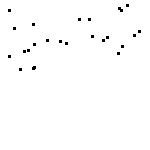
\includegraphics[width=\columnwidth]{figures/04_25_s_nocost.png}}
        \caption{(c)}
        \label{fig_instances_3}
      \end{subfigure} 
       
       \caption{Figures (a)-(c) show 3 out of 60 random instances for experiments. The instances differ in number and size of obstacles and are used for local costmap creation.}
      \label{fig:fig_instances}
   \end{figure}
   
\begin{figure}[thpb]
     \footnotesize
      \centering
      \setlength\fboxsep{0pt}
      \setlength\fboxrule{0.5pt}
       \def\svgwidth{0.7\textwidth}
       %\fbox{\includesvg{figures/fig_inst_25_new}}
       \includesvg{figures/fig_inst_25_new}
		\caption{This figure shows three applications of the local planner in a simulated experiment. The greyscale background image visualizes obstacle costs of a generated costmap. Trajectories in green are drive-able, whereas red trajectories collide with obstacles. In each local planning step possible trajectories are weighted with respect to obstacle closeness and progression towards goal destination. For example in the second step a longer valid trajectory is rejected, while a shorter trajectory which stays farther away from obstacles is selected for execution. After three local planning applications the robot safely reaches the goal destination.}
		\label{fig:fig_instances_detail}
\end{figure}

The following list shows the tested algorithm:
\begin{itemize}
\item{\bf{Random Search with Tabu List:}} A repeated random guess of a velocity tuple $(v,w)$ (RST).
\item{\bf{Iterated Local Search:}} Performing Iterated Local Search with 4, 8 ,and 16 neighbors and Tabu List (ILS4, ILS8, ILS16).
\item{\bf{Variable Neighborhood Search:}} Variable Neighborhood search with Best-,and First-Improvement heuristic, and Tabu List (VNSB, VNSF).
\end{itemize}

\section{Test results}\label{sec:testresults}
All tests were performed on a 2.4 GHz, Intel Core 2 Duo processor using 4 GB RAM. 

In the first experiment the algorithm were applied to all 60 instances to evaluate a broad spectrum of possible environments. 
Figure~\ref{fig:fig_allworlds} illustrates the results using 240 trajectories, and using 2400 trajectory samples.
   \begin{figure}[thpb]
        \footnotesize
      \centering
      \def\svgwidth{0.7\textwidth}
      \includesvg{figures/fig_allworlds}
      \caption{This figure shows the results of testing all 60 randomly generated instances. The top figure shows the run time performance for 240 trajectories, and the bottom figure for 2400 trajectories. Compared to brute force search, the Meta-Heuristic algorithm show a significant improvement. }
      \label{fig:fig_allworlds}
   \end{figure}

 
The results show that all algorithm, including RST, outperform the Brute Force generate-and-test method significantly. 
As expected increasing the number of trajectories greatly favors the Meta-Heuristic algorithm, since they benefit from larger search spaces. 
Notice that ILS and VNS algorithm differ apparently from the RST by exhibiting much smaller variance in their test results, indicating that randomization alone is not enough to achieve very good and stable performance.
Furthermore the VNS exhibit a more stable performance than the ILS methods. 
Comparing the ILS algorithm reveals the connection of the search space size to the size of the neighborhood. 
A small number of trajectories benefits smaller sized neighborhoods, whereas increasing the number of trajectories benefits larger neighborhoods. 

The following tests only include the VNSF, VNSB and ILS4 algorithm. 
The algorithm are executed with specific world instances, and repeated 50 times. 
The results in Figure~\ref{fig:fig_special} show again that the VNS algorithm significantly outperform the Brute Force method. 

\begin{figure}[thb]
   \captionsetup[subfigure]{labelformat=empty} 
   \begin{subfigure}{0.7\textwidth}
        \footnotesize
      \centering
      \def\svgwidth{\columnwidth}
      \includesvg{figures/fig_6_40}
      \caption{(a)}
      \label{fig:fig_6_40}
    \end{subfigure}
    
    \begin{subfigure}{0.7\textwidth}  
      \footnotesize
      \centering
      \def\svgwidth{\columnwidth}
      \includesvg{figures/fig_12_80}
      \caption{(b)}
      \label{fig:fig_12_80}
    \end{subfigure}
    \caption{The results of 50 consecutively executions with (a) 240 and (b) 960 trajectories, on particular instances which differ in number and size of obstacles. The blue line marks the run time for brute force search, which is used as a benchmark.}  
     \label{fig:fig_special}
\end{figure}

%\begin{figure}[thpb]
%     \footnotesize
%      \centering
%      
%      \setlength\fboxsep{0pt}
%      \setlength\fboxrule{0.5pt}
%      \captionsetup[subfigure]{labelformat=empty}   
%      \begin{subfigure}[thpb]{0.45\columnwidth}
%       \def\svgwidth{\columnwidth}
%       \includesvg{figures/15_3_b_6_40}
%       \caption{(a)}
%      \end{subfigure}
%      \begin{subfigure}[thpb]{0.45\columnwidth}
%       \def\svgwidth{\columnwidth}
%       \includesvg{figures/15_3_b_12_80}
%       \caption{(b)}
%      \end{subfigure} 
%               
%      \begin{subfigure}[thpb]{0.45\columnwidth}
%       \def\svgwidth{\columnwidth}
%       \includesvg{figures/30_5_m_6_40}
%       \caption{(c)}
%      \end{subfigure}
%      \begin{subfigure}[thpb]{0.45\columnwidth}
%       \def\svgwidth{\columnwidth}
%       \includesvg{figures/30_5_m_12_80}
%       \caption{(d)}
%      \end{subfigure} 
%           
%      \begin{subfigure}[thpb]{0.45\columnwidth}
%       \def\svgwidth{\columnwidth}
%       \includesvg{figures/45_25_s_6_40}
%       \caption{(e)}
%      \end{subfigure}
%      \begin{subfigure}[thpb]{0.45\columnwidth}
%       \def\svgwidth{\columnwidth}
%       \includesvg{figures/45_25_s_12_80}
%       \caption{(f)}
%      \end{subfigure}   
%      
%       \caption{The results of 50 consecutively executions with 240 (a,c,e) and 960 (b,d,f) trajectories on instances with one obstacle and a size of 1 meter, (a,b), 5 obstacles, 0.5 meter (c,d), and 25 obstacles, 0.1 meter (e,f). The blue line marks the run time for brute force search, which is used as a benchmark.}
%      \label{fig:fig_instances}
%   \end{figure}
   
Analyzing the results of the ILS4 algorithm shows that a too small environment will quickly degrade to random search. 
Here the use of a neighborhood structure pays off and the VNS approaches perform evidently better than ILS. 
In addition, the results show that the algorithm perform good independent of number and size of obstacles.

As for nearly all optimization problems, the No Free Lunch theorems \cite{wolpert1997no} apply to the local planning domain. 
Looking at all the results, there is no clear winner among the algorithm. 
Nevertheless using Variable Neighborhood search with Tabu List and Best Improvement heuristic seem to yields the best and most stable overall performance. 

In general the run time of the python implementation is not very efficient compared to tuned C++ implementations. 
Therefore the absolute numbers of the run time evaluations should be handled with care. 

\section{Conclusions}

Applying Meta-Heuristic search to trajectory selection of local planners like DWA is a first step in using the power of these search procedures in the context of local planning.
The results of our experiments in Section~\ref{sec:testresults} show, that already the small selection using Iterated Local Search, and Variable Neighborhood Search provide significant performance improvement. 
Therefore it would be of interest to investigate related algorithm like GRASP \cite{feo1995grasp}, reduced VNS, or Simulated Annealing \cite{Kirkpatrick83SimulatedAnnealing}. 
In addition, developing more sophisticated neighborhood structures, and extending the tabu search method would also be valuable.

The proposed method is also applicable for robot models of higher degree of freedom, since dealing with large trajectory samples is a particular strength of Meta-Heuristic search.

The applicability to similar path-planning methods using trajectory samples, like Curvature Velocity Method \cite{simmons1996curvature}, or the Trajectory Rollout method implemented in \texttt{move\_base}, are also subject of further investigations. 

One of the next goals is to integrate this trajectory selection in existing planning systems for robots using ROS and analyze the performance of the algorithm using state of the art methods for costmap calculations and collision testing. 
With the gained data a fine tuned local planner using Meta-Heuristic based search methods can be tested under real and simulated environments.

